\section{Methodology: Finite element analysis}
\label{sec:method}
A FEA model was created in ABAQUS. The geometry is based on dimensions obtained from reference \cite{Wu2018}, with a length of 500mm and a subtended angle of 90\degree. The shell element was extruded with a thickness of 0.1mm. Copper Berrilium was chosen as the material with youngs modululus (E) of 156 GPa \cite{Azomaterials} and a poisson' ratio ($\nu$) of 0.35 \cite{Azomaterials}. A mesh refinement study was conducted, after which the 0.0001m mesh size was chosen using the cantilever displacement as a test against the analytically derived result. The mesh elements were formed using S4R elements. To flatten the boom at the root, the equation \ref{eq:disp} was used to find the displacement needed at every node have a flat row of nodes.
\begin{equation}
  y=R-R\times cos(\theta)  
  \label{eq:disp}
\end{equation}
Where $\theta=\frac{Width}{Radius}$. 
Figure \ref{fig:rootdisp} shows the image of the displacement conditions at the tip. Displacement conditions applied resulting in fully flat section as shown in \ref{fig:case24}. The different widths of the booms are modelled by suppressing the nodes from the outer width. Since there were 48 nodes in the root section, the mesh size across the root was calculated by dividing from the circumference of the root end of the boom. 
%table for summary of properties 
These displacements are further given in appendix. In order to find the effects on the boom for the displacement used, the rotational displacement against the moment observed were used to depict on a graph. This was found by constraining the tip nodes using a single control point via a Multi Point Constraint (MPC) and a beam constraint was used in order to equally apply displacements on the tip. The reference point for the node was set at the centre of the semi circle which was used to apply the rotational condition.  

\begin{table}[!hbt]
    \centering
    \begin{tabular}{|c|c|c|c|c|c|}
    \hline
    \textbf{Length} & \textbf{Thickness} & \textbf{Radius} & \textbf{Meshsize} & \textbf{\begin{tabular}[c]{@{}l@{}}Young's\\ Modulus\end{tabular}} & \textbf{\begin{tabular}[c]{@{}l@{}}Poisson's\\ Ratio\end{tabular}} \\ \hline
    500mm & 0.1mm & 15mm & 0.1mm & 158GPa & 0.35 \\  \hline
    \end{tabular}
    \caption{Summary of FEA model}
    \label{tab:fea}
\end{table}
\begin{figure}[!hbt]
\begin{subfigure}{.5\linewidth}
\centering
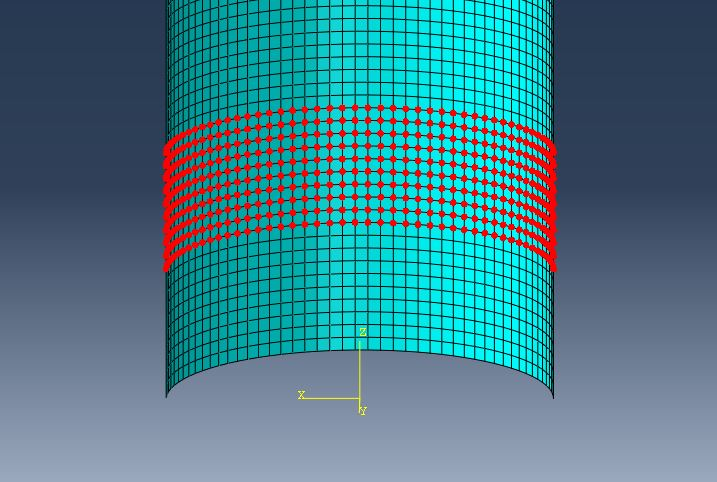
\includegraphics[height=5cm]{images/RootDisp.JPG}
\caption{Displacement conditions required to make the end flat}
\label{fig:rootdisp}
\end{subfigure}%
\begin{subfigure}{.5\linewidth}
\centering
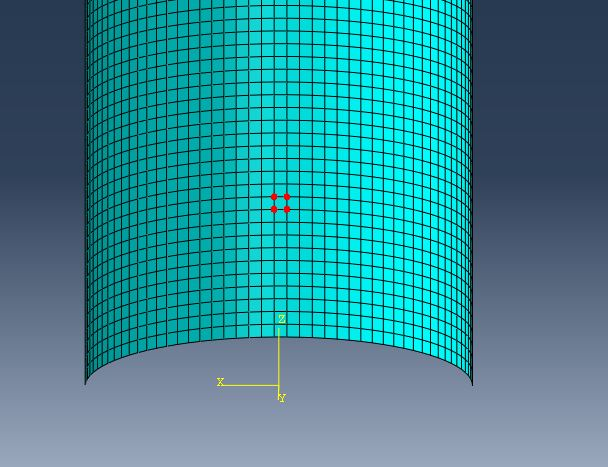
\includegraphics[height=5cm]{images/encastre.JPG}
\caption{Fixed nodes at the root}
\label{fig:sub2}
\end{subfigure}\\[1ex] 
\caption{Displacement conditions applied at the root}
\end{figure}

\begin{figure}
\begin{subfigure}{0.5\linewidth}
\centering
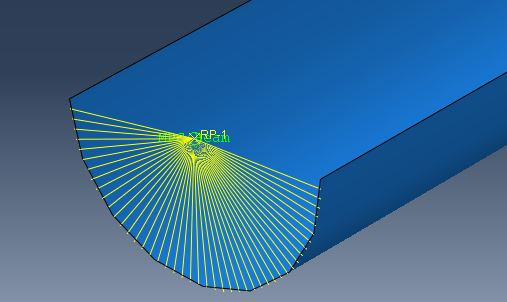
\includegraphics[width=7cm]{images/connectorMPCbeam.JPG}
\caption{MPC connector beam tie linking the nodes in the arc to the reference point using a `Master-Slave' algorithm}
\label{fig:sub3}
\end{subfigure}
\label{fig:test}
\begin{subfigure}{0.5\linewidth}
\centering
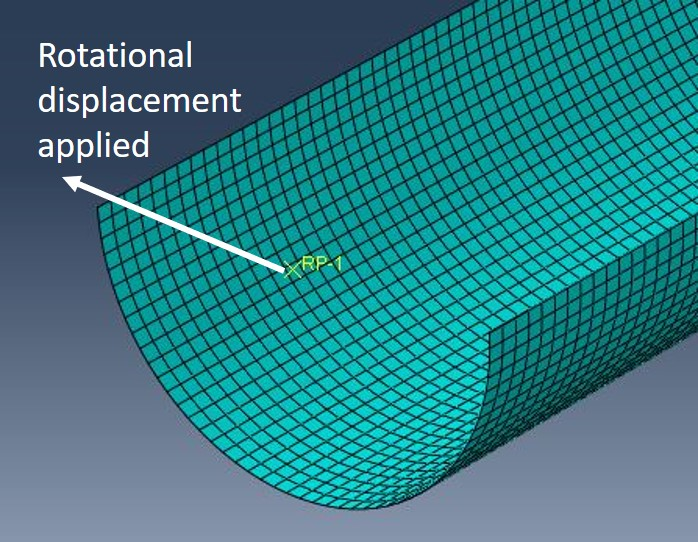
\includegraphics[width=6cm]{images/RP12.jpg}
\caption{Rotational displacement applied to the reference point at the centre of the semi circular arc}
\label{fig:sub3}
\end{subfigure}\\[1ex]
\caption{ABAQUS model tip properties}
\label{fig:test}
\end{figure}
